\documentclass{article}

\usepackage{lmodern}  % for bold teletype font
\usepackage{amsmath}  % for \hookrightarrow
\usepackage{xcolor}   % for \textcolor
\usepackage{listings}
\usepackage{graphicx}

\lstset{
  basicstyle=\ttfamily,
  columns=fullflexible,
  frame=single,
  breaklines=true,
  postbreak=\mbox{\textcolor{red}{$\hookrightarrow$}\space},
}

\title{UCP Report}
\date{\today}
\author{Jakob Wyatt}

\begin{document}

\maketitle
\pagebreak
\tableofcontents
\pagebreak

\section{Purpose of Functions}

This is the call graph of the program:
\begin{figure}[h!]
\label{Program Call Graph}
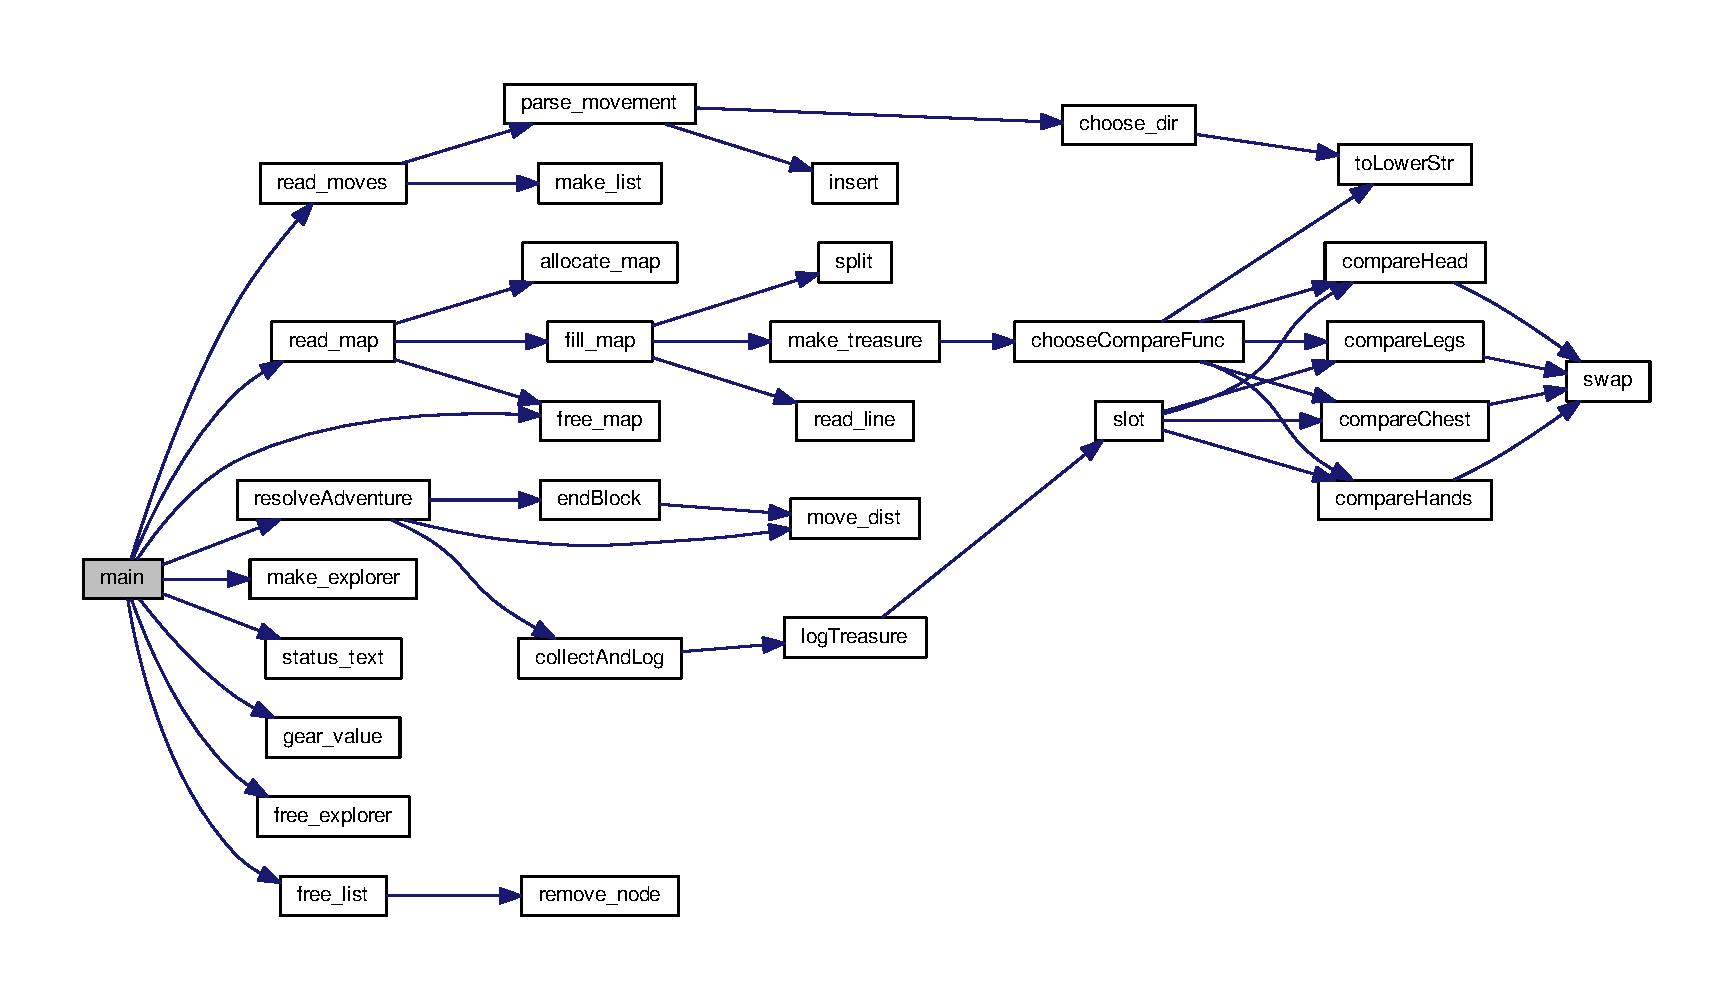
\includegraphics[scale=0.5]{call_graph.pdf}
\end{figure}

\subsection{resolveAdventure}
\begin{lstlisting}
status resolveAdventure(map items, unsigned long rows, unsigned long cols, list movements, explorer* person, FILE* file);
\end{lstlisting}


 Resolve an adventure, given a map and a list of movements.\\ 
 \texttt{items} Map containing all items.\\ 
 \texttt{rows} Number of rows in the map.\\ 
 \texttt{cols} Number of columns in the map.\\ 
 \texttt{movements} Movements to be made by the explorer.\\ 
 \texttt{person} Explorer to collect items.\\ 
 \texttt{file} File to write logs to.\\ 
 \textbf{Return:} SUCCESS if the adventure was sucessful,
         CORRECTED if out of bounds movements were corrected,
         FAILED if out of bounds movements weren't corrected.\\ 
 \textbf{Precondition:}  file must be opened in "a" mode.\\ 
 \textbf{Postcondition:}  items is modified when  treasure is picked up by  person.\\ 
 \textbf{Postcondition:}  items and  movements are not deallocated by this function.
 Define AI to correct out of bounds movements.
         Define LOG to log movements to stdout as well as  file.\\
 \textbf{Implementation:}
Iterate through the list of movements, and keep track of the current location of  person.
This is done in 2 steps:
    \begin{enumerate}
     \item Get the next movement from the list, and calculate the final block  person will be on after this movement.
         This is done with  endBlock.
     \item Travel in the direction of the movement using  moveDist until the final block is reached.
         Treasures are collected and logged with  collectAndLog. 
    \end{enumerate}
 This is done until  movements is exhausted or an error status is set.


\subsection{collectAndLog}
\begin{lstlisting}
void collectAndLog(FILE* file, map items, explorer* person, long i, long j);
\end{lstlisting}


 Collects the treasure at the given location. Logs this event to a file.\\ 
 \texttt{file} File to log information to.\\ 
 \texttt{items} Map containing item to collect.\\ 
 \texttt{person} Explorer to collect the item.\\ 
 \texttt{i} y location of the treasure to collect.\\ 
 \texttt{j} x location of the treasure to collect.\\ 
 \textbf{Precondition:}  file must be opened in "a" mode.\\ 
 \textbf{Postcondition:} The treasure in items is either swapped, destroyed (and deallocated), or retained.\\ 
 
 
 \textbf{Implementation:}
Switch on the type of the treasure.
coin: Deallocate and increase  explorer.coin by  treasure.value.
magic: Deallocate and increase  explorer.magic by  treasure.value.
gear: Use  treasure.compare to compare and conditionally swap the two treasures.
Log with  logTreasure if any deallocation or swapping occured.


\subsection{logTreasure}
\begin{lstlisting}
void logTreasure(FILE* file, treasure x, int collect, long i, long j);
\end{lstlisting}


 Logs a treasure to a file, and optionally stdout.\\ 
 \texttt{file} File to log information to.\\ 
 \texttt{x} Treasure to log.\\ 
 \texttt{collect} If  collect == 0, then log  x as collected.
     Else, log it as discarded.\\ 
 \texttt{i} y location of the treasure.\\ 
 \texttt{j} x location of the treasure.\\ 
 \textbf{Precondition:}  file must be opened in "a" mode.
 Define LOG to write the information to stdout as well as  file.\\ 
 
 
 \textbf{Implementation:}
Switch on  x.type, and log the treasure according to the assignment specification.


\subsection{endBlock}
\begin{lstlisting}
status endBlock(unsigned long rows, unsigned long cols, long* i, long* j, move x);
\end{lstlisting}


 Finds the final block after a movement is performed.\\ 
 \texttt{rows} The number of rows in the map.\\ 
 \texttt{cols} The number of cols in the map.\\ 
 \texttt{i} The starting y location. Exports the new y location.\\ 
 \texttt{j} The starting x location. Exports the new x location.\\ 
 \texttt{x} The movement direction and distance.\\ 
 \textbf{Return:} SUCCESS if the movement was performed correctly,
         CORRECTED if the movement was corrected,
         FAILED if the movement is out of bounds.
 Define AI to correct out of bounds movements.\\ 
 
 
 \textbf{Implementation:}
Move the given distance with  move\_dist.
If AI is defined, correct the location if out of bounds.
If the distance is still out of bounds, return FAILED.


\subsection{move\_dist}
\begin{lstlisting}
void move_dist(direction dir, unsigned long distance, long* i, long* j);
\end{lstlisting}


 Moves a given distance in a given direction.\\ 
 \texttt{dir} The direction to move.\\ 
 \texttt{distance} The distance to move.\\ 
 \texttt{i} The starting y location. Exports the new y location.\\ 
 \texttt{j} The starting x location. Exports the new x location.\\ 
 \textbf{Postcondition:} Does not check if the distance is valid.\\ 
 
 
 \textbf{Implementation:}
Depending on the direction, change the relevant coordinate.


\subsection{insert}
\begin{lstlisting}
void insert(list* x, node* iter, void* data);
\end{lstlisting}


  Insert an element into a linked list.\\ 
 \texttt{x} The list to insert into.\\ 
 \texttt{iter} Insert before this element. If  iter is NULL,
     insert at the end of the list.\\ 
 \texttt{data} The pointer to data that will be stored by the node.\\ 
 
 
 \textbf{Implementation:}
 A node named new is dynamically allocated (on the heap),
     and  data is referenced by it.
     \begin{itemize}
 \item If  iter == NULL, insert at the end of the list.
    \begin{enumerate}
     \item Node before new is  x$\rightarrow$tail.
     \item Node after new is NULL.
     \item  x$\rightarrow$tail is now new.
     \item If there are currently no elements in the list,
             set x$\rightarrow$head to new. Otherwise, link the node before
             new to new.
    \end{enumerate}
 \item Otherwise, the next node is guarenteed to exist.
    \begin{enumerate}
     \item Node before new is  iter$\rightarrow$prev.
     \item Node after new is iter.
     \item  iter$\rightarrow$prev is new.
     \item If iter$\rightarrow$prev is NULL (start of list),  x$\rightarrow$head is new.
         Otherwise, new$\rightarrow$prev$\rightarrow$next is new.
    \end{enumerate}
 \end{itemize}

\subsection{remove\_node}
\begin{lstlisting}
void remove_node(list* x, node* iter);
\end{lstlisting}


  Remove a node from a linked list.\\ 
 \texttt{x} The list to remove the node from.\\ 
 \texttt{iter} The node to remove.
  Calls  free() on  iter.data\\ 
 
 
 \textbf{Implementation:}
First, free  iter$\rightarrow$data.
If  iter is the first element in  x,
 change the head pointer to  iter$\rightarrow$next.
Otherwise, the previous node.next is equal to the
 next node.
When  iter is the final element in  x,
 perform the algorithm above but set the tail pointer
 and the next node.prev instead.
 

\subsection{make\_list}
\begin{lstlisting}
list make_list();
\end{lstlisting}


  Initializes an empty list.\\ 
 \textbf{Return:} The empty list.
  The list struct is statically allocated (on the stack).\\ 
 
 
 \textbf{Implementation:}
Set head and tail to NULL.
 

\subsection{free\_list}
\begin{lstlisting}
void free_list(list* x);
\end{lstlisting}


  Free all elements in the list.\\ 
 \texttt{x} The list to free.
  Calls  free() on  node.data for all nodes.\\ 
 
 
 \textbf{Implementation:}
Call  remove\_node on  x$\rightarrow$head until x$\rightarrow$head is NULL (list is empty).
 

\subsection{for\_each}
\begin{lstlisting}
void for_each(list x, data_func func);
\end{lstlisting}


  Applies a function to every  node in the  list.\\ 
 \texttt{x} The list to apply  func to.\\ 
 \texttt{func} The function to apply to every node.
   func is called on each  node in order.\\ 
 
 
 \textbf{Implementation:}
 \begin{enumerate}
\item Apply  func to the current node, starting at  x.head.
\item Move the current node forward.
\end{enumerate}
Repeat this until the current node is NULL.
 


\subsection{read\_map}
\begin{lstlisting}
status read_map(map* read_into, long* rows, long* cols, char* filename);
\end{lstlisting}


  Reads in a map from a file.\\ 
 \texttt{read\_into} Pointer to the created map.\\ 
 \texttt{rows} The number of rows in the map.\\ 
 \texttt{cols} The number of cols in the map.\\ 
 \texttt{filename} The name of the file to read into.\\ 
 \textbf{Return:} If an error occurs, returns ABORTED. Otherwise,
     returns COMPLETE.\\ 
 \textbf{Postcondition:}  read\_into must be deallocated with  free\_map.
  Writes to stderr if an error has occured. Only deallocate  read\_into
     if this function returns COMPLETE.\\ 
 
 
 \textbf{Implementation:}
This function performs the majority of file opening, size determination, and allocation.
If there is an error in any of the stages listed below, perform any neccesary cleanup
 and exit the function.
 \begin{enumerate}
\item Open the file in "r" mode.
\item Read the size of the map.
\item Allocate the map with  allocate\_map.
\item Read values into the map with  fill\_map.
\end{enumerate}
 

\subsection{allocate\_map}
\begin{lstlisting}
map allocate_map(size_t rows, size_t cols);
\end{lstlisting}


  Allocates a map dynamically (on the heap).\\ 
 \texttt{rows} The number of rows in the map.\\ 
 \texttt{cols} The number of columns in the map.\\ 
 \textbf{Return:} The allocated map. This is NULL if allocation failed.\\ 
 \textbf{Postcondition:}  free\_map must be called on the returned map if it is not NULL.\\ 
 
 
 \textbf{Implementation:}
The map consists of an array of arrays. Allocate the top level array first.
If this was successful, then allocate rows one at a time.
If row allocation fails at any point, iterate backwards through the row arrays
     that have already been allocated, and free them.
After allocation, set the type of each map element to 'N'. This represents the
     map having no elements, and allows deallocation to work as expected.
 

\subsection{free\_map}
\begin{lstlisting}
void free_map(map x, size_t rows, size_t cols);
\end{lstlisting}


  Deallocates a map that has been created with  allocate\_map.\\ 
 \texttt{x} The map to free.\\ 
 \texttt{rows} The number of rows in the map.\\ 
 \texttt{cols} The number of columns in the map.\\ 
 
 
 \textbf{Implementation:}
The only dynamically allocated element in  treasure is
 the detail string.
First, iterate through the map and deallocate any detail strings
 if the type is either 'G' (gear) or 'M' (magic).
Next, deallocate each row array.
Finally, deallocate the column array.
 

\subsection{fill\_map}
\begin{lstlisting}
status fill_map(map read_into, size_t rows, size_t cols, FILE* file);
\end{lstlisting}


  Fills a map with information from a csv file.\\ 
 \texttt{read\_into} The map to read values into.\\ 
 \texttt{rows} The number of rows in the map.\\ 
 \texttt{cols} The number of columns in the map.\\ 
 \texttt{file} The file to read from.\\ 
 \textbf{Precondition:}  read\_into must be created with  allocate\_map.\\ 
 \textbf{Precondition:}  file must be opened in "r" mode.\\ 
 \textbf{Postcondition:}  file is not closed by this function.\\ 
 \textbf{Return:} If an error occurs, return ABORTED. Otherwise, return COMPLETE.
  Writes to stderr if an error occurs.\\ 
 
 
 \textbf{Implementation:}
Stop reading the file as soon as incorrect formatting is encountered.
While there are still empty map rows:
\begin{enumerate}
 \item Read the current line of the file with  read\_line.
 \item Split the line with  split.
 \item If the correct number of tokens has been read, convert each token
     into a treasure with  make\_treasure and add it to the map.
\end{enumerate}
Any errors are printed to stderr.
Strtok cannot be used for this function, as it skips repeated delimiters.
 

\subsection{read\_line}
\begin{lstlisting}
char* read_line(FILE* file);
\end{lstlisting}


  Reads a line from a file.\\ 
 \texttt{file} The file to read from.\\ 
 \textbf{Return:} The line that has been read from the file.\\ 
 \textbf{Precondition:}  file must be opened in "r" mode.\\ 
 \textbf{Postcondition:}  free must be called on the returned string after use.\\ 
 \textbf{Postcondition:} 
  Reads until a newline or EOF is encountered.
     The newline is not included in the returned string.
     If no characters can be read, an empty string ('\\0') is returned.\\ 
 
 
 \textbf{Implementation:}
 read\_line attemps to read a line from a file using fgets,
     with an initial buffer size of 100. If the last character
     in the string has been overwritten then the buffer is
     assumed to be too small, and a bigger buffer is allocated.
     The file position is then returned to its state at the
     start of the function, and reading is attempted again.
     This process is repeated until the entire line has been read.
Any newline characters in the string are found with strchr, and removed.
 

\subsection{split}
\begin{lstlisting}
status split(char* line, char delim, char** tokens, size_t tokens_sz);
\end{lstlisting}


  Splits a string into tokens, seperated by the given delimiter.\\ 
 \texttt{line} The string to split.\\ 
 \texttt{delim} The delimiter to split the string on.\\ 
 \texttt{tokens} An array of char*.
     Each element in the array points to a null-terminated token string.
     These tokens are "stored" in  line.\\ 
 \texttt{tokens\_sz} The size of  tokens.\\ 
 \textbf{Return:} If the amount of potential tokens in  line does not equal
      tokens\_sz, return ABORTED. Otherwise, return COMPLETE.\\ 
 \textbf{Postcondition:}  line should not be read after splitting.
  The delimiter is not included in a token.
     If multiple delimiters occur in order,
         the corresponding tokens are empty strings.
     The lifetime of  tokens is equal to the lifetime of  line.\\ 
 
 
 \textbf{Implementation:}
The gist of this function is quite simple, although the implementation
becomes more complex as error checking is introduced.
At its core, this algorithm:
\begin{enumerate}
 \item Finds the next delimiter in  line.
 \item Assigns the location of the delimiter in  line to '\\0'.
 \item Adds a new element to  tokens, located 1 after the delimiter.
         This is the start of the next token.
\end{enumerate}

Now, assume that the above algorithm ends when either:
\begin{itemize}
 \item The end of the string has been reached.
 \item The token array is full.
\end{itemize}

If the number of tokens is less than tokens\_sz, there are too few tokens
in  line and the algorithm ends with status ABORTED.
However, if the number of tokens is equal to tokens\_sz, it is not yet known
     if all delimiters have been found or not. To resolve this, find the next
     character that is either a delimiter or a null terminator.
If it is a null terminator, then we have read the correct number of tokens,
 and the algorithm ends with status COMPLETE.
If it is a delimiter, we still have token(s) we have not read yet,
 and the algorithm ends with status ABORTED.
 

\subsection{print\_map}
\begin{lstlisting}
void print_map(map x, size_t rows, size_t cols);
\end{lstlisting}


  Prints a map to stdout.\\ 
 \texttt{x} The map to print.\\ 
 \texttt{rows} The number of rows in the map.\\ 
 \texttt{cols} The number of columns in the map.
  Used for debugging purposes.\\ 
 
 
 \textbf{Implementation:}
Iterate through the map, printing each treasure using  print(treasure).
Also print information about the location of the treasure (row and column).
 

\subsection{read\_moves}
\begin{lstlisting}
status read_moves(list* moves, char* filename);
\end{lstlisting}


  Reads moves from a file into a linked list.\\ 
 \texttt{moves} The list to read moves into.\\ 
 \texttt{filename} The filename to read from.\\ 
 \textbf{Return:} If the file contains incorrect formatting, return ABORTED.
     Otherwise, return COMPLETE.\\ 
 \textbf{Precondition:}  moves is created with  make\_list.\\ 
 \textbf{Postcondition:}  moves must be deallocated with  free\_list, regardless
     of the return status of this function.
  If the file contains incorrect formatting, print a message
     to stderr.\\ 
 
 
 \textbf{Implementation:}
First, open the file in "r" mode. Then, read and process each line until EOF is reached.
The maximum valid line size is 29 characters long, as the largest valid integer representation
in c is 22 characters long.
(+ 5 characters for RIGHT direction, +1 character for space, +1 for null-terminator).
Use  fgets to read a line of the file into this buffer.  parse\_movement is then
 used to parse the line and add the movement to  moves.
 

\subsection{parse\_movement}
\begin{lstlisting}
status parse_movement(list* moves, char* line);
\end{lstlisting}


  Parse a line of movement and add it to the list.\\ 
 \texttt{moves} The list to read the movement into.\\ 
 \texttt{line} The line to read from.\\ 
 \textbf{Return:} If there is an error in the line, return ABORTED.
     Otherwise, return COMPLETE.\\ 
 \textbf{Precondition:}  line must be null-terminated, and must not be NULL.
  This function modifies  moves on faliure, and therefore
     does not have strong exception safety. If there is an error
     in the line, a message is printed to stderr.\\ 
 
 
 \textbf{Implementation:}
First, allocate space for the move and add it to the end of  moves.
Doing this early on reduces the chance memory safety is programmed incorrectly.
Modifying  moves is okay, as strong exception safety is not guarenteed by this function.

Next, check for a space in the line.
This is the seperator between the direction and the distance.
If there are no spaces in the line, the string is incorrectly formatted and the algorithm ends.

Finally, parse the direction with  choose\_dir
 and the distance with  sscanf, and check for errors.
 

\subsection{choose\_dir}
\begin{lstlisting}
direction choose_dir(char* dir);
\end{lstlisting}


  Converts a string to a  direction.\\ 
 \texttt{dir} The string describing the direction.\\ 
 \textbf{Return:} The direction represented by  dir. If the direction is invalid,
     return INVALID.\\ 
 \textbf{Precondition:}  dir must be null-terminated, and must not be NULL.\\ 
 \textbf{Postcondition:}  dir is converted to lowercase in this process.\\ 
 
 
 \textbf{Implementation:}
First, convert the string to lowercase.
Next, use a simple else-if ladder to choose the correct direction.
 

\subsection{direction\_to\_string}
\begin{lstlisting}
void direction_to_string(direction d, char* str);
\end{lstlisting}


  Converts a direction to an uppercase string.\\ 
 \texttt{d} The direction to convert.\\ 
 \texttt{str} The string to write the direction to.\\ 
 \textbf{Postcondition:}  str must be able to hold at least 8 characters.\\ 
 
 
 \textbf{Implementation:}
Use a simple else-if ladder to determine the direction,
 and print the corresponding string into  str.
Another method of implementing this would be to create an
array linking enumerations to strings.
 

\subsection{print\_move}
\begin{lstlisting}
void print_move(void* m);
\end{lstlisting}


  Prints a move to stdout.\\ 
 \texttt{m} A pointer to the  move to print.
   m is a void* so that this function is compatible with  for\_each.
     Used for debugging purposes.\\ 
 
 
 \textbf{Implementation:}
Convert the direction to a string with  direction\_to\_string,
 and print both the direction and distance to stdout.
 

\subsection{main}
\begin{lstlisting}
int main(int argc, char* argv[])
\end{lstlisting}


  The entry point of the program.\\ 
 \texttt{argc} The number of command line arguments.
     The first argument is the name of the program.\\ 
 \texttt{argv} The command line arguments.\\ 
 \textbf{Return:} 0
  Implements functionality described in the assignment brief.
 

\subsection{make\_treasure}
\begin{lstlisting}
status make_treasure(char* str, treasure* make);
\end{lstlisting}


  Parses  str to create a treasure object.\\ 
 \texttt{str} The string to parse.\\ 
 \texttt{make} The created treasure.\\ 
 \textbf{Precondition:}  str must be null-terminated, and must not be NULL.\\ 
 \textbf{Precondition:}  make must be dynamically allocated (on the heap) before calling this function.\\ 
 \textbf{Postcondition:} If  str is empty,  make$\rightarrow$type == 'N'.\\ 
 \textbf{Return:} If the string is invalid, return ABORTED.
     Otherwise, return COMPLETE.
  If the string is invalid, print an error message to stderr.
     Negative treasure values are valid. This is so that negative effects can be impemented.
     For example, if an explorer stumbles across a potion that ends up being a poison,
     their magic value is reduced. Likewise, negative coins could be valid if the explorer
     is robbed by bandits.\\ 
 
 
 \textbf{Implementation:}
The first character in the string is the type of  treasure.
\begin{itemize}
\item If the type is 'C' (coin), then read in the value of the treasure.
\item If the type is 'M' (magic), then:
\begin{enumerate}
     \item Find the first colon in the string.
     \item Copy the detail string from  str + 2 to the seperator.
         This skips the type character, and the space after the type character.
     \item Parse the value, located at one past the seperator to the end of  str.
\end{enumerate}
\item If the type is 'G' (gear), then:
\begin{enumerate}
     \item Find both delimiters ':' in the string.
     \item Copy the detail string from  str + 2 to the seperator.
     \item Find the gear slot with  chooseCompareFunc. This is located between the two seperators.
     \item Parse the value, located at one past the second seperator to the end of  str.
\end{enumerate}
\item If the type is '\\0', then  str is empty and the type of treasure is 'N' (none).
\end{itemize}

\subsection{swap}
\begin{lstlisting}
void swap(treasure* a, treasure* b);
\end{lstlisting}


  Swaps two treasures.\\ 
 \texttt{a} The first treasure to swap.\\ 
 \texttt{b} The second treasure to swap.\\ 
 \textbf{Precondition:}  a and  b must not be NULL.\\ 
 
 
 \textbf{Implementation:}
Create a temporary variable and use it to swap the two values.
 

\subsection{chooseCompareFunc}
\begin{lstlisting}
compare_func chooseCompareFunc(char* str);
\end{lstlisting}


  Chooses a compare function given a body part.\\ 
 \texttt{str} The string representing a body part.\\ 
 \textbf{Return:} A function pointer to the correct compare function.\\ 
 \textbf{Postcondition:} If  str is invalid, return NULL.\\ 
 
 
 \textbf{Implementation:}
First, convert the string to lowercase.
Next, use a simple else-if ladder to determine
which  compare\_func to use.
 

\subsection{slot}
\begin{lstlisting}
void slot(treasure x, char* str);
\end{lstlisting}


  Writes the textual representation of the gear slot into the string.\\ 
 \texttt{x} The treasure containing the gear slot.\\ 
 \texttt{str} The string to write the representation into.\\ 
 \textbf{Precondition:}  str must be able to hold at least 6 characters.
  If  x.type != 'G', do not modify  str.\\ 
 
 
 \textbf{Implementation:}
Use a simple else-if ladder to determine which string to use,
comparing the  x.compare function pointer.
 

\subsection{toLowerStr}
\begin{lstlisting}
void toLowerStr(char* str);
\end{lstlisting}


  Converts the given string to lowercase.\\ 
 \texttt{str} The string to convert to lowercase.\\ 
 
 
 \textbf{Implementation:}
Iterate through the string, using  tolower to convert
each character to lowercase.
 

\subsection{print}
\begin{lstlisting}
void print(treasure x);
\end{lstlisting}


  Prints a treasure to stdout.\\ 
 \texttt{x} The treasure to print.
  Used for debugging. If  x.type == 'N',
     do not print anything.\\ 
 
 
 \textbf{Implementation:}
If the type is 'N', do not print anything.
All non-empty  treasures have types and values.
These are printed.
If the type is not 'C' (coin), the treasure has a detail string.
This is printed.
If the type is 'G' (gear), print the slot it refers to.
     This uses  slot to convert  x.compare into a string.
 

\subsection{compareHead}
\begin{lstlisting}
int compareHead(treasure* gear, explorer* person);
\end{lstlisting}


  Implementation of  compare\_func for the head slot.\\ 
 
 
 \textbf{Implementation:}
If  person$\rightarrow$head.value is less than  gear.value,
use  swap to swap the objects.
 

\subsection{compareChest}
\begin{lstlisting}
int compareChest(treasure* gear, explorer* person);
\end{lstlisting}


  Implementation of  compare\_func for the head slot.\\ 
 
 
 \textbf{Implementation:}
Same as  compareHead, except the Chest slot is compared instead.
 

\subsection{compareLegs}
\begin{lstlisting}
int compareLegs(treasure* gear, explorer* person);
\end{lstlisting}


  Implementation of  compare\_func for the head slot.\\ 
 
 
 \textbf{Implementation:}
Same as  compareHead, except the Legs slot is compared instead.
 

\subsection{compareHands}
\begin{lstlisting}
int compareHands(treasure* gear, explorer* person);
\end{lstlisting}


  Implementation of  compare\_func for the head slot.\\ 
 
 
 \textbf{Implementation:}
Same as  compareHead, except the Hands slot is compared instead.
 

\subsection{make\_explorer}
\begin{lstlisting}
explorer make_explorer();
\end{lstlisting}


  Creates an explorer.\\ 
 \textbf{Return:} An explorer with no magic, coin, or gear.\\ 
 
 
 \textbf{Implementation:}
Initialize magic and coin to 0.
Initialize gear.type to 'N'.
Initialize gear.value to -1, so that when compared
the empty slot is always initially swapped.
 

\subsection{free\_explorer}
\begin{lstlisting}
void free_explorer(explorer ex);
\end{lstlisting}


  Frees any memory owned by the explorer.\\ 
 \texttt{ex} The explorer to free.\\ 
 
 
 \textbf{Implementation:}
If gear.type == 'G' (non-empty), free the corresponding detail string.
 

\subsection{gear\_value}
\begin{lstlisting}
int gear_value(explorer ex);
\end{lstlisting}


  Finds the total value of all gear owned by the explorer.\\ 
 \texttt{ex} The explorer to calculate the total value of all gear for.\\ 
 \textbf{Return:} The total value of all gear.\\ 
 \textbf{Precondition:}  ex must be created with  make\_explorer.\\ 
 
 
 \textbf{Implementation:}
If gear.type == 'G' (there is gear in that slot),
increment the accumulator by that gear's value.
 

\subsection{status\_text}
\begin{lstlisting}
void status_text(status s, char* text_rep);
\end{lstlisting}


  Converts the status to text.\\ 
 \texttt{s} The status to convert.\\ 
 \texttt{text\_rep} The location to print the status string.\\ 
 \textbf{Precondition:}  text\_rep must be able to hold at least 10 characters.\\ 
 
 
 \textbf{Implementation:}
Simple else-if ladder to read the correct string
into  text\_rep.

\section{Conversion of Input File to Coordinate System}
\subsection{Implementation}
The top level function to convert the input file is read\_map.
This function opens the file, reads and validates the map size (rows and columns),
and uses allocate\_map to allocate memory for the map.

Once this is done, fill\_map is called.
This function parses the file line by line, and reads values into the map.
First, read\_line is called. This function reads a line of arbitrary size
by reallocating larger buffers until the line is read in full. This means that
the map can be as large as the user wants.
Once the line is read, it is split into tokens using split. This function iterates
over the provided string, finds a given delimiter (',' in this case) with strchr, and substitutes
it will a null-terminator. It then exports an array filled with pointers to the start
of each token. This has the effect of breaking a string up into many substrings, seperated
by the delimiter.

Once this is done, each individual token is passed to make\_treasure. This function
uses a switch statement on the first character to determine the type of the treasure.
Once the type is determined, the treasure is usually parsed by finding the colon character(s)
with strchr, and either using strncpy or sscanf to parse each section.
In the case of a gear treasure,
the function chooseCompareFunc is used to determine which function pointer should be used
with the given slot.

\subsection{Alternate Implementation}

An alternate approach would be to either use strtok, or the given tokenizer, to parse each line.
This would mean that make\_treasure would be passed tokens one at a time, rather than splitting the entire
string and then passing all tokens to make\_treasure. This method was not chosen, as strtok ignores repeated
characters and is therefore unsuitable for any empty sections of the map. strtok could also be used to parse
individual treasures, instead of using strchr.


\section{Sample Input and Output}
All test results are generated from the TreasureHunter binary.
This is called with the arguments:
\begin{lstlisting}
    ./TreasureHunter <map file> <list file>
\end{lstlisting}
A script to run these tests is located in test/all\_tests.sh.
There is no user input for any test cases.
If example output from adventure.log is not provided, it should be assumed that the binary
does not provide log file output for that test case.

The TreasureHunterLog binary will produce the same output as the TreasureHunter binary,
except any output to the log file (adventure.log) is also output to stdout. This is done
real time; as lines are printed to the log file, the same content is printed to stdout.

The TreasureHunterAI binary is assumed to produce the same output as the TreasureHunter binary,
unless otherwise stated.

\subsection{Example Input from Assignment Brief}
\quad \textbf{Map}
\begin{lstlisting}
5,4
,,C 200,
,G Vibranium Shield:hands:990,,C 50
M Healing Potion:85,,M Defence Enchantment:360,
,,,
,,G Lightsaber:hands:850,
\end{lstlisting}

\textbf{List}
\begin{lstlisting}
DOWN 2
RIGHT 2
DOWn 2
up 0
LEFT 1
UP 3
riGHT 0
RIGHT 2
\end{lstlisting}
\pagebreak

\textbf{stdout}
\begin{lstlisting}
STATUS: COMPLETE
COINS: 50
MAGIC: 445
GEAR: 990
\end{lstlisting}

\textbf{Log file}
\begin{lstlisting}
---
COLLECT<ITEM:MAGIC, XLOC:2, YLOC:0, DESCRIPTION:Healing Potion, VALUE:85>
COLLECT<ITEM:MAGIC, XLOC:2, YLOC:2, DESCRIPTION:Defence Enchantment, VALUE:360>
COLLECT<ITEM:GEAR, XLOC:4, YLOC:2, DESCRIPTION:Lightsaber, SLOT:hands, VALUE:850>
COLLECT<ITEM:GEAR, XLOC:1, YLOC:1, DESCRIPTION:Vibranium Shield, SLOT:hands, VALUE:990>
DISCARD<ITEM:GEAR, XLOC:1, YLOC:1, DESCRIPTION:Lightsaber, SLOT:hands, VALUE:850>
COLLECT<ITEM:COINS, XLOC:1, YLOC:3, VALUE:50>
\end{lstlisting}

\subsection{Out of Bounds}
\subsubsection{TreasureHunter}
\quad \textbf{Map}
\begin{lstlisting}
7,3
,g Thorn armour:CheST:120,C 200
,G Vibranium Shield:hands:990,
M Healing Potion:85,,M Defence Enchantment:360
,m Phoenix Blood:291,
,g IDEK_ANYMORE:heaD:21,G Lightsaber:hAnDs:850
c 350,g Crimson Plate:cHeSt:1020,
,G Infinity Pants:leGS:30000,
\end{lstlisting}

\textbf{List}
\begin{lstlisting}
LEFt 3
RIGHT 1
down 2
LEfT 5
RIGHT 20
left 1
DOWN 100
UP 2000
\end{lstlisting}
\pagebreak

\textbf{stdout}
\begin{lstlisting}
STATUS: FAILED
\end{lstlisting}

\textbf{Log file}
\begin{lstlisting}
---
\end{lstlisting}

\subsubsection{TreasureHunterAI}
\quad \textbf{Map}
\begin{lstlisting}
7,3
,g Thorn armour:CheST:120,C 200
,G Vibranium Shield:hands:990,
M Healing Potion:85,,M Defence Enchantment:360
,m Phoenix Blood:291,
,g IDEK_ANYMORE:heaD:21,G Lightsaber:hAnDs:850
c 350,g Crimson Plate:cHeSt:1020,
,G Infinity Pants:leGS:30000,
\end{lstlisting}

\textbf{List}
\begin{lstlisting}
LEFt 3
RIGHT 1
down 2
LEfT 5
RIGHT 20
left 1
DOWN 100
UP 2000
\end{lstlisting}
\pagebreak

\textbf{stdout}
\begin{lstlisting}
STATUS: CORRECTED
COINS: 0
MAGIC: 736
GEAR: 32031
\end{lstlisting}

\textbf{Log file}
\begin{lstlisting}
---
COLLECT<ITEM:GEAR, XLOC:0, YLOC:1, DESCRIPTION:Thorn armour, SLOT:chest, VALUE:120>
COLLECT<ITEM:GEAR, XLOC:1, YLOC:1, DESCRIPTION:Vibranium Shield, SLOT:hands, VALUE:990>
COLLECT<ITEM:MAGIC, XLOC:2, YLOC:0, DESCRIPTION:Healing Potion, VALUE:85>
COLLECT<ITEM:MAGIC, XLOC:2, YLOC:2, DESCRIPTION:Defence Enchantment, VALUE:360>
COLLECT<ITEM:MAGIC, XLOC:3, YLOC:1, DESCRIPTION:Phoenix Blood, VALUE:291>
COLLECT<ITEM:GEAR, XLOC:4, YLOC:1, DESCRIPTION:IDEK_ANYMORE, SLOT:head, VALUE:21>
COLLECT<ITEM:GEAR, XLOC:5, YLOC:1, DESCRIPTION:Crimson Plate, SLOT:chest, VALUE:1020>
DISCARD<ITEM:GEAR, XLOC:5, YLOC:1, DESCRIPTION:Thorn armour, SLOT:chest, VALUE:120>
COLLECT<ITEM:GEAR, XLOC:6, YLOC:1, DESCRIPTION:Infinity Pants, SLOT:legs, VALUE:30000>
\end{lstlisting}

\subsection{Empty List}
\quad \textbf{Map}
\begin{lstlisting}
5,4
,,C 200,
,G Vibranium Shield:hands:990,,C 50
M Healing Potion:85,,M Defence Enchantment:360,
,,,
,,G Lightsaber:hands:850,
\end{lstlisting}

\textbf{List}
\begin{lstlisting}

\end{lstlisting}
\pagebreak

\textbf{stderr}
\begin{lstlisting}
File <list file> was empty.
\end{lstlisting}

\subsection{Invalid Direction}
\quad \textbf{Map}
\begin{lstlisting}
5,4
,,C 200,
,G Vibranium Shield:hands:990,,C 50
M Healing Potion:85,,M Defence Enchantment:360,
,,,
,,G Lightsaber:hands:850,
\end{lstlisting}

\textbf{List}
\begin{lstlisting}
LEFT 3
riGhtt 1
DOWN 2
LEFT 5
RIGHT 20
NOrtH 1
DOWN 100
UP 2000
\end{lstlisting}
\pagebreak

\textbf{stderr}
\begin{lstlisting}
Invalid direction
At line 2.
\end{lstlisting}

\subsection{Invalid Distance}

\quad \textbf{Map}
\begin{lstlisting}
5,4
,,C 200,
,G Vibranium Shield:hands:990,,C 50
M Healing Potion:85,,M Defence Enchantment:360,
,,,
,,G Lightsaber:hands:850,
\end{lstlisting}

\textbf{List}
\begin{lstlisting}
DOWN 2
RIGHT 2
DOWn %s
up 0
LEFT 1
UP 3
riGHT 0
RIGHT 2
\end{lstlisting}
\pagebreak

\textbf{stderr}
\begin{lstlisting}
Distance must be an integer
At line 3.
\end{lstlisting}

\subsection{No Space in List}

\quad \textbf{Map}
\begin{lstlisting}
5,4
,,C 200,
,G Vibranium Shield:hands:990,,C 50
M Healing Potion:85,,M Defence Enchantment:360,
,,,
,,G Lightsaber:hands:850,
\end{lstlisting}

\textbf{List}
\begin{lstlisting}
DOWN 2
RIGHT 2
DOWn 2
up 0
LEFT1
UP 3
riGHT 0
RIGHT 1
\end{lstlisting}
\pagebreak

\textbf{stderr}
\begin{lstlisting}
No space
At line 5.
\end{lstlisting}

\subsection{Negative Distance}

\quad \textbf{Map}
\begin{lstlisting}
5,4
,,C 200,
,G Vibranium Shield:hands:990,,C 50
M Healing Potion:85,,M Defence Enchantment:360,
,,,
,,G Lightsaber:hands:850,
\end{lstlisting}

\textbf{List}
\begin{lstlisting}
DOWN 2
RIGHT 2
DOWn 2
up 0
LEFT 1
UP 3
riGHT 0
RIGHT -100
\end{lstlisting}
\pagebreak

\textbf{stderr}
\begin{lstlisting}
Distance must be positive
At line 8.
\end{lstlisting}

\subsection{Floating Point Distance}

\quad \textbf{Map}
\begin{lstlisting}
5,4
,,C 200,
,G Vibranium Shield:hands:990,,C 50
M Healing Potion:85,,M Defence Enchantment:360,
,,,
,,G Lightsaber:hands:850,
\end{lstlisting}

\textbf{List}
\begin{lstlisting}
DOWN 2
RIGHT 2
DOWn 2
up 0
LEFT 1
UP 3
riGHT 0.5
RIGHT 100
\end{lstlisting}
\pagebreak

\textbf{stderr}
\begin{lstlisting}
Distance must be an integer
At line 7.
\end{lstlisting}

\subsection{Empty Map}

\quad \textbf{Map}
\begin{lstlisting}

\end{lstlisting}

\textbf{List}
\begin{lstlisting}
DOWN 2
RIGHT 2
DOWn 2
up 0
LEFT 1
UP 3
riGHT 0
RIGHT 2
\end{lstlisting}
\pagebreak

\textbf{stderr}
\begin{lstlisting}
Incorrect formatting in <map file>, line 1: Expected positive integers <rows>,<cols>
\end{lstlisting}

\subsection{Incorrect Rows}

\quad \textbf{Map}
\begin{lstlisting}
7,3
,g Thorn armour:CheST:120,C 200
,G Vibranium Shield:hands:990,
M Healing Potion:85,,M Defence Enchantment:360
,m Phoenix Blood:291,
,g IDEK_ANYMORE:heaD:21,G Lightsaber:hAnDs:850
c 350,g Crimson Plate:cHeSt:1020,
\end{lstlisting}

\textbf{List}
\begin{lstlisting}
DOWN 2
RIGHT 2
DOWn 2
up 0
LEFT 1
UP 3
riGHT 0
RIGHT 2
\end{lstlisting}
\pagebreak

\textbf{stderr}
\begin{lstlisting}
Incorrect number of rows: read 6, expected 7.
\end{lstlisting}

\subsection{Incorrect Columns}

\quad \textbf{Map}
\begin{lstlisting}
7,3
,g Thorn armour:CheST:120,C 200
,G Vibranium Shield:hands:990,
M Healing Potion:85,,M Defence Enchantment:360
,m Phoenix Blood:291,
,g IDEK_ANYMORE:heaD:21,G Lightsaber:hAnDs:850
c 350,g Crimson Plate:cHeSt:1020
,G Infinity Pants:leGS:30000,
\end{lstlisting}

\textbf{List}
\begin{lstlisting}
DOWN 2
RIGHT 2
DOWn 2
up 0
LEFT 1
UP 3
riGHT 0
RIGHT 2
\end{lstlisting}
\pagebreak

\textbf{stderr}
\begin{lstlisting}
Incorrect number of columns at line 7: expected 3.
\end{lstlisting}

\subsection{Negative Columns}

\quad \textbf{Map}
\begin{lstlisting}
7,-3
,g Thorn armour:CheST:120,C 200
,G Vibranium Shield:hands:990,
M Healing Potion:85,,M Defence Enchantment:360
,m Phoenix Blood:291,
,g IDEK_ANYMORE:heaD:21,G Lightsaber:hAnDs:850
c 350,g Crimson Plate:cHeSt:1020,
,G Infinity Pants:leGS:30000,
\end{lstlisting}

\textbf{List}
\begin{lstlisting}
DOWN 2
RIGHT 2
DOWn 2
up 0
LEFT 1
UP 3
riGHT 0
RIGHT 2
\end{lstlisting}
\pagebreak

\textbf{stderr}
\begin{lstlisting}
Incorrect formatting in <map file>, line 1: Expected positive integers <rows>,<cols>
\end{lstlisting}

\subsection{Invalid Rows}

\quad \textbf{Map}
\begin{lstlisting}
7.5,3
,g Thorn armour:CheST:120,C 200
,G Vibranium Shield:hands:990,
M Healing Potion:85,,M Defence Enchantment:360
,m Phoenix Blood:291,
,g IDEK_ANYMORE:heaD:21,G Lightsaber:hAnDs:850
c 350,g Crimson Plate:cHeSt:1020,
,G Infinity Pants:leGS:30000,
\end{lstlisting}

\textbf{List}
\begin{lstlisting}
DOWN 2
RIGHT 2
DOWn 2
up 0
LEFT 1
UP 3
riGHT 0
RIGHT 2
\end{lstlisting}
\pagebreak

\textbf{stderr}
\begin{lstlisting}
Incorrect formatting in <map file>, line 1: Expected positive integers <rows>,<cols>
\end{lstlisting}

\subsection{Invalid Treasure Type}

\quad \textbf{Map}
\begin{lstlisting}
7,3
,g Thorn armour:CheST:120,C 200
,G Vibranium Shield:hands:990,
M Healing Potion:85,,M Defence Enchantment:360
,m Phoenix Blood:291,
,g IDEK_ANYMORE:heaD:21,f Lightsaber:hAnDs:850
c 350,g Crimson Plate:cHeSt:1020,
,G Infinity Pants:leGS:30000,
\end{lstlisting}

\textbf{List}
\begin{lstlisting}
DOWN 2
RIGHT 2
DOWn 2
up 0
LEFT 1
UP 3
riGHT 0
RIGHT 2
\end{lstlisting}
\pagebreak

\textbf{stderr}
\begin{lstlisting}
F is not a valid treasure type.
At row 5, column 3.
\end{lstlisting}

\subsection{Invalid Slot}

\quad \textbf{Map}
\begin{lstlisting}
7,3
,g Thorn armour:CheST:120,C 200
,G Vibranium Shield:hands:990,
M Healing Potion:85,,M Defence Enchantment:360
,m Phoenix Blood:291,
,g IDEK_ANYMORE:heaD:21,G bow and arrows:feet:850
c 350,g Crimson Plate:cHeSt:1020,
,G Infinity Pants:leGS:30000,
\end{lstlisting}

\textbf{List}
\begin{lstlisting}
DOWN 2
RIGHT 2
DOWn 2
up 0
LEFT 1
UP 3
riGHT 0
RIGHT 2
\end{lstlisting}
\pagebreak

\textbf{stderr}
\begin{lstlisting}
Incorrect formatting. Gear is represented as: "G <detail>:<slot>:<value>"
At row 5, column 3.
\end{lstlisting}

\subsection{Invalid Value}

\quad \textbf{Map}
\begin{lstlisting}
7,3
,g Thorn armour:CheST:120,C 200
,G Vibranium Shield:hands:99.5,
M Healing Potion:85,,M Defence Enchantment:360
,m Phoenix Blood:291,
,g IDEK_ANYMORE:heaD:21,G Lightsaber:hAnDs:850
c 350,g Crimson Plate:cHeSt:1020,
,G Infinity Pants:leGS:30000,
\end{lstlisting}

\textbf{List}
\begin{lstlisting}
DOWN 2
RIGHT 2
DOWn 2
up 0
LEFT 1
UP 3
riGHT 0
RIGHT 2
\end{lstlisting}
\pagebreak

\textbf{stderr}
\begin{lstlisting}
Incorrect formatting. Gear is represented as: "G <detail>:<slot>:<value>"
At row 2, column 2.
\end{lstlisting}

\subsection{Too Many Colons}

\quad \textbf{Map}
\begin{lstlisting}
7,3
,g Thorn armour:CheST:120,C 200
,G Vibranium Shield:hands:990,
M Healing:Potion:85,,M Defence Enchantment:360
,m Phoenix Blood:291,
,g IDEK_ANYMORE:heaD:21,G Lightsaber:hAnDs:850
c 350,g Crimson Plate:cHeSt:1020,
,G Infinity Pants:leGS:30000,
\end{lstlisting}

\textbf{List}
\begin{lstlisting}
DOWN 2
RIGHT 2
DOWn 2
up 0
LEFT 1
UP 3
riGHT 0
RIGHT 2
\end{lstlisting}
\pagebreak

\textbf{stderr}
\begin{lstlisting}
Incorrect formatting. Magic items are represented as: "M <detail>:<value>"
At row 3, column 1.
\end{lstlisting}

\subsection{Too Little Colons}

\quad \textbf{Map}
\begin{lstlisting}
7,3
,g Thorn armour:CheST:120,C 200
,G Vibranium Shield:hands:990,
M Healing Potion:85,,M Defence Enchantment:360
,m Phoenix Blood:291,
,g IDEK_ANYMORE:heaD:21,G Lightsaber:hAnDs:850
c 350,g Crimson Plate:cHeSt:1020,
,G Infinity Pants leGS:30000,
\end{lstlisting}

\textbf{List}
\begin{lstlisting}
DOWN 2
RIGHT 2
DOWn 2
up 0
LEFT 1
UP 3
riGHT 0
RIGHT 2
\end{lstlisting}
\pagebreak

\textbf{stderr}
\begin{lstlisting}
Incorrect formatting. Gear is represented as: "G <detail>:<slot>:<value>"
At row 7, column 2.
\end{lstlisting}

\subsection{No Space in Map}

\quad \textbf{Map}
\begin{lstlisting}
7,3
,g Thorn armour:CheST:120,C 200
,G Vibranium Shield:hands:990,
MHealing Potion:85,,M Defence Enchantment:360
,m Phoenix Blood:291,
,g IDEK_ANYMORE:heaD:21,G Lightsaber:hAnDs:850
c 350,g Crimson Plate:cHeSt:1020,
,G Infinity Pants:leGS:30000,
\end{lstlisting}

\textbf{List}
\begin{lstlisting}
DOWN 2
RIGHT 2
DOWn 2
up 0
LEFT 1
UP 3
riGHT 0
RIGHT 2
\end{lstlisting}
\pagebreak

\textbf{stderr}
\begin{lstlisting}
Incorrect formatting. Magic items are represented as: "M <detail>:<value>"
At row 3, column 1.
\end{lstlisting}

\end{document}
